

\begin{document}



\chapter*{Введение}

%Включение введения в соодержание
\addcontentsline{toc}{chapter}{Введение}

Для осуществления монетарной политики Центральный Банк может использовать не только традиционные инструменты, но и словесные интервенции (open mouth operations). Суть словесных интервенций очень хорошо иллюстрирует история, которая произошла в США в 1970-1980 гг., в эпоху, которая вошла в мировую историю как Великая инфляция. 

В 1958 г. была опубликована статья экономиста Филиппса, в которой он обнаружил достаточно четкую отрицательную связь между инфляцией и безработицей в Англии за прошедшие 70 лет. Проверка этой работы на американских данных подтвердила взаимосвязь. Кривую Филиппса стали интерпретировать как некую возможность выбора между высокой инфляцией и высокой безработицей~\cite{phillips1958relation}.

Любому политику безработица кажется более значимой социальной проблемой, нежели инфляция и он хочет ее победить любыми доступными средствами. Самым популярным средством по борьбе с безработицей является экспансионистская монетарная политика, состоящая в расширении денежной массы. Именно это и было сделано президентом США Ричардом Никсоном в начале 1970-х гг. в ходе погони за низкой безработицей и высокой инфляцией.

К сожалению, план Никсона удался только наполовину, он добился высокой инфляции, но сбить безработицу не смог, а кривая Филиппса в этот период перестала существовать. 

Все западные страны так или иначе поэкспериментировали с кривой Филиппса и в итоге обрекли 1980-е гг. на обуздание высокой инфляции.

В 1979 г. главой ФРС становится Пол Волкер, который принимает решение очень жестко бороться с инфляцией, однако экономические агенты не верят в заявления ФРС и продолжают ожидать высоких темпов инфляции. Пол Волкер увеличивает процентные ставки и отправляет экономику в краткосрочную рецессию, тем самым сбивая ожидания и уменьшая инфляцию в течение своего председательства с 11,22\% до 3,66\%. 

Таким образом, Пол Волкер заслужил репутацию принципиального борца с высокой инфляцией. Общество верило в его обещания, и при каком-либо макроэкономическом шоке ему достаточно было просто подать сигнал о намерении что-то сделать, и общество сразу же перестраивало свои ожидания в соответствии с этим сигналом.

Таким образом ФРС, заработав устойчивую репутацию, оставляла неизменной величину традиционных инструментов, однако целевые переменные изменялись именно в том направлении, которое требовалось ФРС.

Будем подразумевать под информационными интервенциями сигналы, которые подает Центральный банк для того, чтобы достичь определенного уровня целевой переменной при неизменных величинах традиционных инструментов.

На первый взгляд, речь о возможности регулирования экономики посредством информационных интервенций кажется полным абсурдом, однако существуют центральные банки, которые успешно применяют этот инструмент на практике. Примером такого центрального банка является Резервный Банк Новой Зеландии~(РБНЗ)~\cite{guthrie2000open}.

Целью данной работы является проверка гипотезы влияния словесных интервенций Банка России на динамику валютного курса и процентной ставки. Для достижения цели были поставлены задачи: 

\begin{enumerate}
\item провести критический обзор теоретических работ для выявления механизма воздействия словесных интервенций на динамику макроэкономических переменных;

\item провести критический анализ эмпирических подходов, применяемых для исследования влияния словесных интервенций на динамику различных макроэкономических переменных;

\item собрать и предварительно обработать статистические данные, необходимые для проведения собственных расчетов;

\item построить и оценить модели для проверки влияния словесных интервенции на динамику ставки процента и валютного курса;

\item сформулировать выводы о работоспособности словесных интервенций как инструмента монетарной политики в России.
\end{enumerate}

В первой главе работы будут рассмотрены теоретические работы, освещающие механизмы влияния центральных банков на макроэкономику посредством сигналов.

Во второй главе будут рассмотрены эмпирические работы. После изучения существующих в научной среде подходов к оценке эффективности словесных интервенций как инструмента монетарной политики будет сделан выбор в пользу одного из подходов для проверки работоспособности интервенций на российских данных. 

В третьей главе будут поставлены гипотезы для исследования, осуществлен сбор данных и проведена проверка поставленных гипотез. В заключении будут приведены основные итоги исследования.

%%% Возвращаем нормальную нумерацию глав! 
\titleformat{\chapter} 
    {\normalfont\bfseries\large}
    {\chaptertitlename~\thechapter}{1 em}{\normalfont\bfseries}
    
    
\chapter{Теоретические исследования влияния словесных интервенций на динамику макроэкономических переменных}

\section{Будущее монетарной политики: центральный банк как армия \\ сигнальщиков}

В 1999 году в июле в Оксфорде проходила конференция «Социальные науки и будущее», на которой выступил Бенджамин Фридман\footnote{This paper was initially prepared for the conference on «Social Science and the Future» held at Oxford, U.K., July 7-8, 1999.}. 

Фридман говорил об угрозах и вызовах, которые коснутся монетарной политики в течение первой четверти нового века. Он поднял на обозрение достаточно большое количество проблем, с которыми  центральные банки будут вынуждены столкнуться, и поставил под сомнение возможность проведения монетарной политики в том виде, в котором она присутствует в макроэкономике сегодня. 
 
 Фридман отметил, что публичные заявления различных ЦБ и другие более тонкие сигналы с их стороны приводят к немедленным изменениям цен и доходностей на финансовых рынках, которые в свою очередь приводят к изменению других экономических переменных: 
 
«Сегодня, действительно, широко распространено мнение, которое заключается в том, что центральные банки ровным счетом ничего не должны делать. После достаточно четкого заявления ЦБ о своих намерениях, рынок сделает всю работу~за~него»~\cite{friedman1999future}.

\section{Словесные интервенции Центрального Банка}
Вслед за Фридманом многие авторы начали активно изучать область информационных сигналов. В таких работах авторы, используя теоретико-игровой подход для описания взаимодействия центрального банка и общества пришли к выводу, что заявления, выпущенные ЦБ, и выступления их глав в парламентах оказывают существенное влияние на рыночные процентные ставки, стоимости активов и валютный курс. 

Этот отклик происходит в следствие того, что ЦБ предоставляет в ходе таких выступлений важную информацию о своих ближайших политических предпочтениях и перспективах экономики. 

\section{Информационный канал}

Осуществление монетарной политики происходит через чёрный ящик монетарной политики: каналы монетарной трансмиссии.

К традиционным каналам монетарной трансмиссии относят процентный и валютный. Кроме того существую банковские каналы, значимость которых ввиду развития финансовых рынков и борьбой с рыночными несовершенствами падает. В последнее время в развитых странах, где процентный канал постепенно перестает функционировать, возрастает роль информационного канала монетарной трансмиссии.

\section{Теоретико-игровой подход в моделировании словесных интервенций}

Большая часть теоретических моделей, описывающих различные словесные интервенции, реализуют теоретико-игровой подход. В играх такого рода взаимодействуют центральный банк и общество. Общество формирует ожидания, а центральный банк --- величину целевой переменной.

\subsection{Модель Кинланда и Прескота}

Уровень инфляции в экономике напрямую связано с предложением денег. Центробанк вынужден искать золотую середину между уменьшением безработицы и экономическим ростом, к которым может привести увеличение предложения денег, и  издержками от инфляции. Эта взаимосвязь задается кривой Филиппса:

\begin{equation}\label{T3-1}
y = \bar y + b(\pi-\pi^e),
\end{equation}
где $y$ --- ВВП, $\pi$ --- инфляция, $\pi^e$ --- ожидаемый уровень инфляции, $\bar y$ --- потенциальный ВВП.
 
Пусть ВВП и инфляция определяются в результате следующей игры. На первом этапе этой игры общество формирует свои инфляционные ожидания. На втором этапе ЦБ определяет уровень инфляции и предложение денег в экономике. 
Функция полезности ЦБ представляет собой функцию социальных потерь вида:

\begin{equation}\label{T3-2}
U_b = -(y - y^0)^2 - \alpha (\pi - \pi^0)^2.
\end{equation}
Полезность общества зависит от того, насколько точным оказался его прогноз инфляции:

\begin{equation}\label{T3-3}
U_p = -(\pi - \pi^e)^2.
\end{equation}

Найдем равновесие в этой игре при нулевом целевом уровне инфляции. Сначала решим задачу ЦБ при данной ожидаемой инфляции.

\subsection{Репутация центрального банка}

Для того чтобы ЦБ смог успешно осуществлять словесные интервенции, экономические агенты, условно говоря, должны видеть в Центральном банке «угрозу», которая в любой момент может вмешаться в экономику. Для того чтобы быть «угрозой» Центральный банк, безусловно, должен обладать монополией на резервы, однако этого недостаточно. Кроме всего прочего Центральному банку необходима репутация, заработать которую очень сложно. Именно репутационные механизмы задействовал в 1980-х гг. Пол Волкер.

Если ЦБ обладает репутацией беспринципного борца с высокой инфляцией, то общество, доверяя его обещаниям, закладывает в зарплаты низкие инфляционные ожидания. Обманув общество, центральный банк добьется высокого ВВП на какое-то время, но при этом потеряет свою репутацию. 

Теоретико-игровая модель, описывающая репутационные механизмы центрального банка, была предложена Барро~в~1986~г.~\cite{barro1986reputation}.


\subsection{Объявление ЦБ целевых ориентиров} 
Одним из вопросов, обсуждаемых в теоретико-игровой литературе, связанной с моделированием словесных интервенций, является вопрос важности объявления центральным банком своих намерений, выражающихся в фиксировании целевых уровней для ключевых макроэкономических переменных.   
  
Стэфан Палмквист в своей работе отмечает, что тенденцией последнего времени является активный переход различных стран к режиму таргетирования инфляции. Целью своей работы он ставит разработку модели, которая помогла бы понять как центральный банк может оказывать на экономику влияние за счет объявления своих целей или намерений. Конструируя свою модель на основе работ Кинланда и Прескота, Барро и Гордона, автор пытается объяснить, почему центральные банки иногда объявляют свои цели и намерения частному сектору, а иногда~нет~\cite{palmqvist1998central}. 

\subsection{Неоднозначность прозрачности деятельности ЦБ}

Сегодня любой центральный банк должен нести ответственность за свои решения и соответствовать самым высоким стандартам порядочности и компетентности. Любое решение, принимаемое независимым центральным банком, преследующем свои непосредственные цели, должно носить максимально прозрачный характер. Мало кто ставит под сомнение то, что в таком широком смысле ЦБ должен быть прозрачным. Однако в научной литературе ведутся активные дебаты, связанные с прозрачностью деятельности ЦБ в узком смысле. 


\chapter{Эмпирические исследования влияния словесных интервенций на экономику}

В этой главе будут рассмотрены эмпирические работы, посвященные исследованию функционирования информационного канала и применению словесных интервенций как инструмента монетарной политики. 

Тема словесных интервенций в монетарной политике является относительно новой. Однако несмотря на её новизну, к сегодняшнему дню сформировалось огромное количество различных подходов к работе со словесными интервенциями.

Отдельно стоит отметить, что в большинстве работ, представленных в данном обзоре и  проверяющих наличие влияния словесных интервенций на динамику различных макроэкономических переменных, все оценки заявлений, сделанных центральными банками, делаются экспертно и, в определенном смысле, носят достаточно субъективный характер.

Обобщенные результаты критического анализа эмпирических работ приведены в таблице~\ref{tab1}.


\begin{longtable}{|m{2.5cm}|m{3.5cm}|m{2.5cm}|m{6cm}|}
	\caption{Критические выводы обзора эмпирических работ}\label{tab1}\\
	\hline
	Авторы & Выборка & Метод & Результат исследования \\ 
	\endfirsthead
	\multicolumn{4}{r}{Окончание таблицы \ref{tab1}}\\\hline
	Авторы & Выборка & Метод & Результат исследования \\ \hline
	\endhead
	\hline
	\endfoot
	\hline
	\endlastfoot
\hline
  		Дэниэл Тронтон, 2004 & США, дневные данные, 1974-1979 гг. & Процедура Йохансона & Влияние словесных интервенции ФРС на динамику ставок отсутствует  \\
  		\hline
  		Грэми Гатри и Джулиан Райт, 1999 & Новая Зеландия, дневные данные, 1 января 1979 г. - 30 сентября 1997 г.& Структурные VAR & Словесные интервенции влияют на динамику ставок и валютного курса  \\ 
  		\hline
  		Марсель Фатнер, 2008 & США, Германия, Япония, дневные данные с 1990 по 2003 гг.  & Метод максимального правдоподобия, EGARCH & Словесные интервенции являются эффективным инструментом монетарной политики по отношению к валютному курсу \\ 
  		\hline
  		Майкл Эрман и Марсель Фатнер, 2007 & США, Великобритания, Евросоюз, дневные данные с 1997 по 2000 гг. & Метод максимального правдоподобия, EGARCH & Словесные интервенции влияют на динамику процентных ставок \\ 
  		\hline
  		Пол Мизен, 2009 & Евросоюз, дневные данные из работы Стефан Герлах & Тест Песарана-Тиммермана & Гипотеза о том, что заявления ЕЦБ не влияют на изменение ставки, отвергается  \\
  		\hline
  		Дональд Кох и Брайн Сак, 2003 & США, дневные данные 1989 - 2003 гг. & Метод наименьших квадратов & Заявления ФРС влияют на динамику цен на фьючерсы  \\
  		\hline
  		Леонардо Мелоси, 2013 & США, квартальные 1970-2006 гг. & DSGE & Сигналы повышают способность ФРС стабилизировать экономику  \\
  		\hline
  		Хелдэр Ферера и Ивандо Фариаб, 2014 & Бразилия, дневные данные 2004-2009 гг. &Метод максимального правдоподобия, EGARCH& Словесные интервенции ЦБ эффективно влияют на динамику процентной ставки \\
  		\hline
\end{longtable}

В целом, обзор эмпирических работ указывает на наличие влияния словесных интервенций на динамику различных макроэкономических переменных в разных  странах. В изученных работах отклик на изменение переменной, отвечающей за словесные интервенции, оказывается значимым. 

В третьей главе рассмотренные выше подходы будут применены для оценки эффективности словесных интервенций Банка России.


\chapter{Оценка эффективности заявлений Банка России}

\section{Формулировка задач для исследования}

В конце 2014 г. Банк России принял решение перейти к режиму инфляционного таргетирования. Интерес представляет решение следующих двух задач:

\begin{enumerate}

\item[\textbf{Прямая задача:}] Оказывают ли в России словесные интервенции влияние на динамику валютного курса и процентных ставок?

\item[\textbf{Двойственная задача:}] Можно ли по динамике валютного курса или процентной ставки предсказать характер словесной интервенции (ужесточающая или смягчающая)?
\end{enumerate}

\section{Данные}

Выборка охватывает период с 1 января 2015 года по 31 декабря 2015 года. Для решения поставленных задач были использованы дневные данные. 

Все данные о динамике обменного валютного курса (рублей за доллар США)  были взяты из базы данных  «Финам». Значения индекса РТС были взяты с сайта Московской Биржи. При расчётах используются цены на момент закрытия биржи. Процентная ставка МИАКР по кредитам сроком на один день и информация о валютных интервенциях были взяты из базы данных Банка России. Цены на нефть марки Brent были взяты из базы данных «Финам».

Для конструирования дамми-переменной, отвечающей за словесные интервенции использовался новостной архив газеты «Ведомости». На языке программирования Python был написан код, который вытащил из архива все статьи, в заголовках которых фигурировали словосочетания: «Набиулл», «Центробанк», «Юдаев», «Банк России», «ЦБ». Для последующей обработки были сохранены текст каждой статьи, её заголовок и ссылка на неё. Код, использованный для выкачки, приведен в приложении А.  

В ходе изучения статей были сформированы следующие дамми-
переменные:

\begin{enumerate}
\item[] $S=1$, если в рассматриваемый день Банком России было сделано заявление, подразумевающее что в будущем будет произведено ужесточение монетарной политики;

\item[] $S=-1$, если в рассматриваемый день Банком России было сделано заявление, подразумевающее что в будущем будет произведено смягчение монетарной политики;

\item[] $S=0$, если в рассматриваемый день не было сделано ни одного заявления или все заявления носили нейтральный характер.
\end{enumerate}

\begin{table}[h]
	\begin{center}
		\caption{Описание переменных}\label{varieble}
		\begin{tabular}{|m{3cm}|m{8cm}|}
  		\hline
  		Переменная & Описание \\ \hline
    	$USD$ & валютный курс (рублей за доллар)  \\ \hline
  		$RTS$ & индекс РТС \\ \hline
  		$MIACR$ & процентная ставка МИАКР по кредитам сроком на один день \\ \hline
  		$VAL$ & объем валютных интервенций\\ \hline
  		$OIL$ & цены на нефть \\ \hline
  		$D$ & переменная, принимающая значение 1, если рассматриваемый день - первый рабочий день после выходных или последний рабочий день перед выходными \\ \hline
  		$S$ & словесные интервенции (-1--- смягчение, 1 --- ужесточение, 0 --- характер интервенции неясен) \\ \hline
		\end{tabular}
	\end{center}
\end{table}

Всеобъемлющая доступность новостной информации позволяет узнать экономическим агентам о наличии словесных интервенций практически моментально. В связи с этим отклик в целевой переменной должен произойти в тот же день, когда произошла словесная интервенция или на следующий день после словесной интервенции.

\section{Решение двойственной задачи}

Проверим можно ли по динамике валютного курса, ставки процента или индекса РТС предсказать характер заявления, которое делает Банк России. Для этого оценим следующую порядковую пробит-модель:

\begin{equation}
S_t = \begin{cases} -1 &\text{ если } b(L) \Delta X_{t-1} + c(L) S_{t-1} + \varepsilon_t < \gamma_1 \\
\mbox{ }0 &\text{ если } \gamma_1 < b(L) \Delta X_{t-1} + c(L) S_{t-1} + \varepsilon_t < \gamma_2 \\
\mbox{ }1 &\text{ если } \gamma_2 < b(L) \Delta X_{t-1} + c(L) S_{t-1} + \varepsilon_t 
\end{cases}, 
\end{equation}

где $X_{t}$ --- ставка МИАКР, обменный курс или индекс РТС, $\varepsilon_t \sim iid N (0, \sigma^2)$, $b(L) = \sum_{j=1}^m b_j L^j$, $c(L) = \sum_{j=1}^n c_j L^j$.

Модель оценивалась методом максимального правдоподобия. Количество лагов $n$ и $m$ выбиралось с помощью минимизации критерия Шварца из десяти запаздываний для каждой переменной. Перебор показал, что оптимальны значения $n=1$ и $m=1$. Код, с помощью которого производился отбор, приведен в приложении Б. После оценивания с помощью статистики Вальда проверялась гипотеза о незначимости регрессии в целом.

В таблице~\ref{stask} представлены результаты решения двойственной задачи. Каждая из рассмотренных порядковых пробит регрессий незначима на 5\% уровне значимости. Аналогичный результат был получен для динамики цен на нефть. 

\begin{table}[H]
	\begin{center}
		\caption{Решение двойственной задачи}\label{stask}
		\begin{tabular}{|m{6cm}|m{4cm}|}
\hline
Объясняющие переменные & P-значение для проверки гипотезы $b_0 = c_0 =0$  \\ \hline
$\Dt USD_{t-1}$, $S_{t-1}$ & 0.1344   \\ \hline
$\Dt RTS_{t-1}$, $S_{t-1}$ & 0.0715   \\ \hline
$\Dt MIACR_{t-1}$, $S_{t-1}$ & 0.3625   \\ \hline
$\Dt OIL_{t-1}$, $S_{t-1}$ & 0.1302   \\ \hline
		\end{tabular}
	\end{center}
\end{table}

Таким образом гипотеза о том, что динамика переменных, рассмотренных выше, не несёт никакой информации о будущих заявлениях Банка России не отвергается.


\section{Решение прямой задачи с помощью методологии VAR}

Проверим влияют ли словесные интервенции Банка России в течение рассматриваемого периода на динамику валютного курса, процентной ставки и индекса РТС. Для исследования данного вопроса будем использовать методологию VAR.

В работе Гатри и Райта, уже упоминавшейся выше, у РБНЗ имелась цель монетарной политики. ЦБ таргетировал постоянный номинальный запас денежных средств. РБНЗ ежедневно публикует на своём сайте свой прогноз по номинальному запасу денежных средств и учитывает его, осуществляя операции на открытом рынке~\cite{guthrie2000open}. 

В течение рассматриваемого периода Банк России придерживается режима таргетирования инфляции. Вполне уместно было бы специфицировать модель похожим образом, используя вместо ошибок прогноза расчета движения денежных средств отклонение текущего уровня инфляции от таргетируемого. Однако в условиях дневных данных это является невозможным в связи со спецификой расчета инфляции. Попробуем специфицировать модель несколькими различными способами отличными от работы Новозеландских коллег и сравним полученные результаты между собой. Код для оценки соответствующих моделей и построения функций импульсного отклика приведен в приложении В.

\textbf{Первая спецификация:}

\begin{equation}
\left\{
\begin{aligned}
\Dt X_t &= \a + \sum_{i=1}^p \a_{xi} \Dt X_{t-i} + \sum_{i=1}^p \a_{si} S_{t-i} +\a_d D_t +  u_{1t}, \\
S_t &= \b + \sum_{i=1}^p \b_{xi} \Dt X_{t-i} + \sum_{i=1}^p \b_{si} S_{t-i} + \b_d D_t +  u_{2t}.
\end{aligned}
\right.
\end{equation}
 
При оценивании модели количество лагов выбиралось из 10 запаздываний с помощью критерия Шварца. Он показал, что оптимальным является взять одно запаздывание. 

При решении двойственной задачи было получено, что заявления Банка России не зависят от лагированных или одновременных значений процентной ставки МИАКР, валютного курса и индеса РТС. Исходя из этого факта упорядочим переменные как $S_t \to \Dt X_t$.

Функции импульсного отклика валютного курса, индекса РТС и ставки МИАКР на заявление Банка России при такой спецификации и идентифицирующих предположениях будут иметь вид, представленный на рис.~\ref{otkl_1}. Функции импульсного отклика представлены с 95\% доверительными интервалами, построенными с помощью бутстрапа.

\begin{figure}[h]
\begin{minipage}[h!]{0.49\linewidth}
\center{\footnotesize{Валютный курс} \\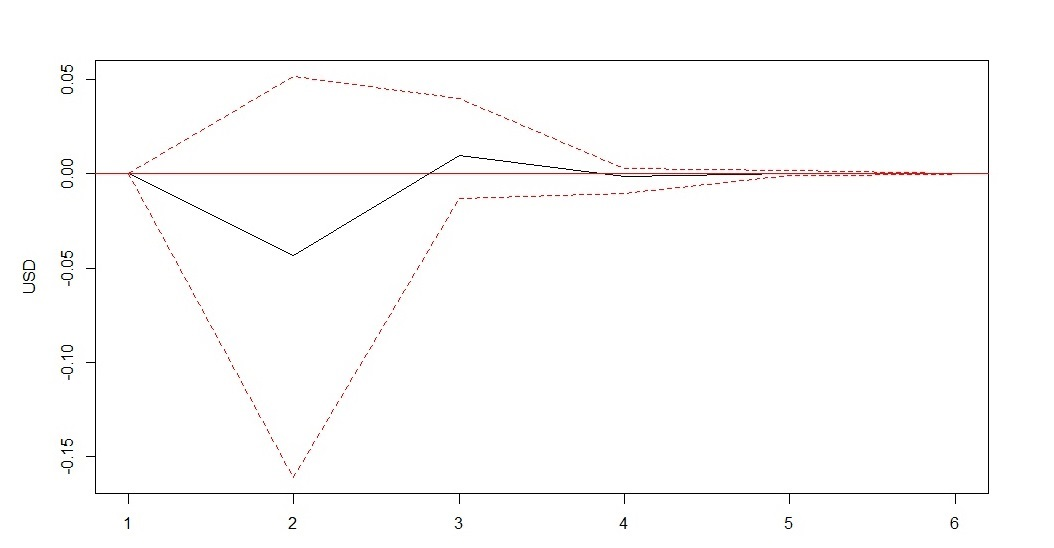
\includegraphics[width=1\linewidth]{1_usd_res}}
\end{minipage}
\hfill
\begin{minipage}[h!]{0.49\linewidth}
\center{\footnotesize{Индекс РТС} \\ 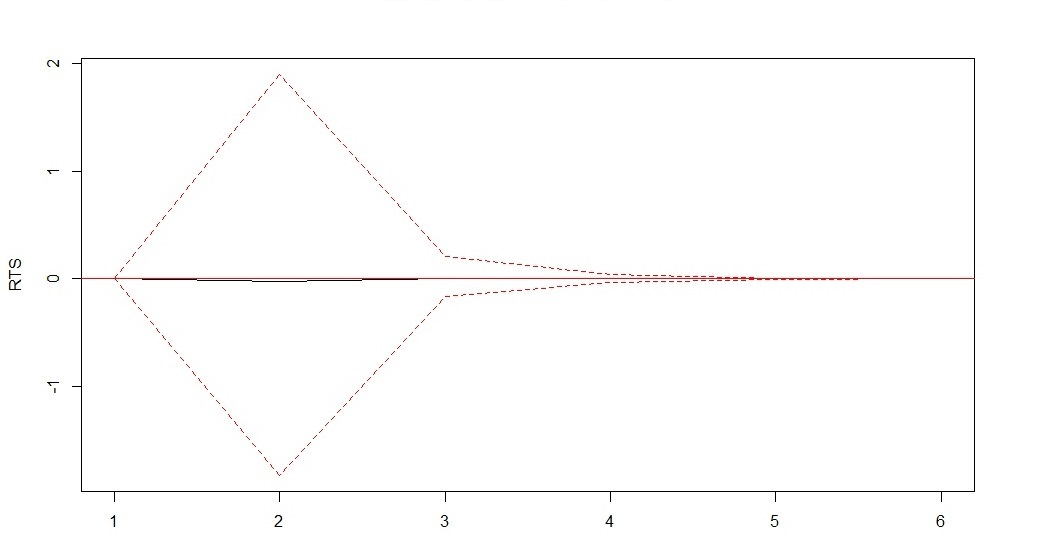
\includegraphics[width=1\linewidth]{1_rts_res}}
\end{minipage}
\vfill
\begin{minipage}[h!]{0.49\linewidth}
\center{\footnotesize{Однодневная ставка МИАКР} \\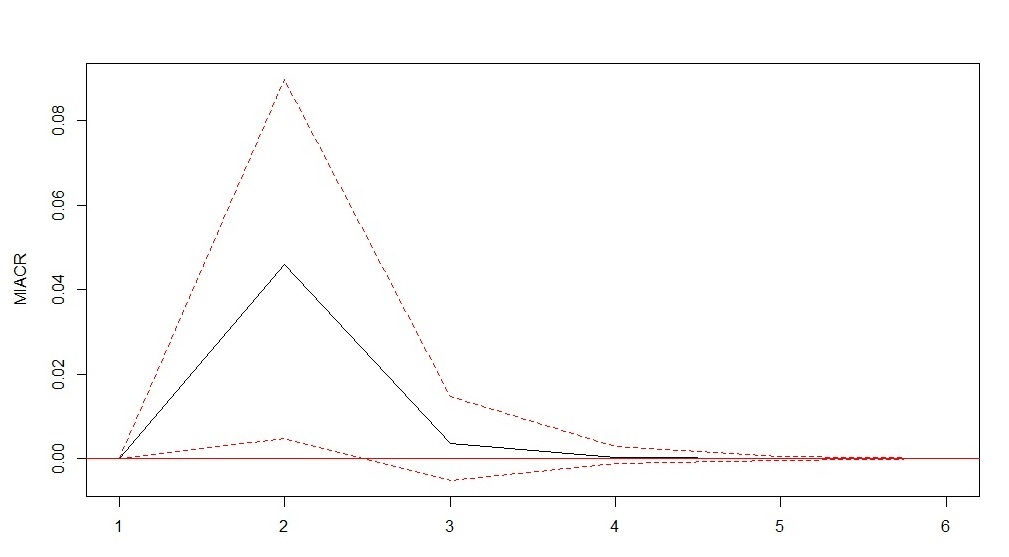
\includegraphics[width=1\linewidth]{1_miacr_res}} 
\end{minipage}
\caption{Функции импульсного отклика валютного курса, индекса РТС и ставки МИАКР на заявления Банка России}
\label{otkl_1}
\end{figure}

Из представленных графиков видно, что отклики валютного курса и индекса РТС на заявления Банка России незначимы. При этом, при ужесточающем заявлении, происходит шок в процентной ставке МИАКР. 

%%% Оформляем Заключение и список литературы также как Оглавление и Введение

\titleformat{\chapter} 
    {\normalfont\bfseries\large}
    {\noindent}{0em}{\centering\normalfont\bfseries}  


\chapter*{Заключение}
\addcontentsline{toc}{chapter}{Заключение}

Начиная с 2014 г. Банк России, в связи с переходом к режиму инфляционного таргетирования, начал иначе перестраивать свою информационную политику, повышая уровень предсказуемости и прозрачности. Управление ожиданиями постепенно налаживается, однако в Центробанке отмечают, что уровень репутации, необходимый для эффективного использования информационного канала, ещё не достигнут. 

В данной работе были рассмотрены различные методы анализа влияния словесных интервенций на динамику различных макроэкономических переменных. С их помощью был проведён анализ информационной политики Банка России.  

В работе была сделана попытка ответить на два вопроса: «Оказывают ли в России словесные интервенции влияние на динамику валютного курса, индекса РТС и процентных ставок?» и «Можно ли по динамике валютного курса, индекса РТС или процентной ставки предсказать характер словесной интервенции?». 

В результате оценки порядковой пробит модели было получено, что нет никаких свидетельств статистической предсказуемости словесных интервенций. 

С помощью методологии VAR были построены функции импульсного отклика валютного курса, индекса РТС и ставки процента на словесные интервенции Банка России. Отклики индекса РТС и валютного курса оказались незначимы для всех рассмотренных спецификаций. Отклик однодневной процентной ставки на заявления Банка России МИАКР оказался значимым. При ужесточающем заявлении происходит рост ставки на 0.04 базовых пункта. Такое изменение процентной ставки является несущественным. Использование методологии GARCH и теста Песарана-Тимермана подтвердили, полученные с помощью методологии VAR результаты. В течение 2015 года словесные интервенции не оказывали влияния на динамику вышеперечисленных макроэкономических переменных. 

\newpage


%Если вашей душе мил bibtex и вы разберетесь как работать с пакетом bibtex-gost, то эта команда для вас!
%\printbibliography

%Команда для нормального названия у списка литры!
\renewcommand\bibname{Список литературы}

\begin{thebibliography}{99}
\addcontentsline{toc}{chapter}{Список литературы}%добавляем в соодержание

\bibitem{UDAEVA} Юдаева, К. В. О денежно-кредитной политике Банка России на современном этапе //Деньги и кредит. –- 2014. –- С. 13.

\bibitem{barro1986reputation} Barro, R. J. Reputation in a model of monetary policy with incomplete information //Journal of Monetary Economics. –- 1986. -- Т. 17. №. 1. С. 3-20.

\bibitem{barro1981positive} Barro, R. J., Gordon, D. B. A positive theory of monetary policy in a natural-rate model. –- 1981.

\bibitem{boivin2010has} Boivin J., Kiley M. T., Mishkin F. S. How has the monetary transmission mechanism evolved over time?. – National Bureau of Economic Research -- 2010.-– №. w15879.

\bibitem{cook1989effect} Cook T., Hahn T. The effect of changes in the federal funds rate target on market interest rates in the 1970s //Journal of Monetary Economics. –- 1989. –- Т. 24. №. 3. С. 331-351.


\bibitem{ehrmann2007communication} Ehrmann M., Fratzscher M. Communication by central bank committee members: Different strategies, same effectiveness? //Journal of Money, Credit and Banking. –- 2007. –- Т. 39. №. 2-3. С. 509-541.

\bibitem{fratzscher2008communication} Fratzscher M. Communication and exchange rate policy //Journal of Macroeconomics. -- 2008. -– Т. 30. №. 4. С. 1651-1672.

\bibitem{friedman1999future} Friedman B. M. The future of monetary policy: the central bank as an army with only a signal corps? //International finance. -– 1999. –- Т. 2. №. 3. С. 321-338.

\bibitem{gerlach2007interest} Gerlach S. et al. Interest rate setting by the ECB, 1999-2006: Words and deeds //International Journal of Central Banking. –- 2007. –- Т. 3. №. 3. С. 1-46.

\bibitem{guthrie2000open} Guthrie G., Wright J. Open mouth operations //Journal of Monetary Economics. –- 2000. -– Т. 46. №. 2. С. 489-516.

\bibitem{hayek1945use} Hayek F. A. The use of knowledge in society //The American economic review. –- 1945. -- С. 519-530.

\bibitem{kohn2003central} Kohn D. L. et al. Central bank talk: does it matter and why?//Divisions of Research \& Statistics and Monetary Affairs, Federal Reserve Board -- 2003.

\bibitem{kydland1977rules} Kydland F. E., Prescott E. C. Rules rather than discretion: The inconsistency of optimal plans //The journal of political Economy. –- 1977. –- С. 473-491.MLA	


\bibitem{melosi2013signaling} Melosi L. Signaling effects of monetary policy. –- 2013.

\bibitem{de2015brazilian} ГОСТ	
de Mendonça H. F., Faria I. Brazilian Central Bank communication and interest rate expectations //Macroeconomics and Finance in Emerging Market Economies. -– 2015. -- Т. 8. №. 1-2. С. 25-44.

\bibitem{mizen2009can} Mizen P. What can we learn from central bankers' words? Some nonparametric tests for the ECB //Economics Letters. –- 2009.-– Т. 103. №. 1. С. 29-32.

\bibitem{morris2005central} Morris S., Shin H. S. Central bank transparency and the signal value of prices //Brookings Papers on Economic Activity. -– 2005. -– Т. 2005. №. 2. С. 1-66.

\bibitem{palmqvist1998central} Palmqvist S. Why Central Banks Announce their Objectives: Monetary Policy with Discretionary Signalling. -- 1998.

\bibitem{pesaran2000recursive} Pesaran M. H., Timmermann A. A recursive modelling approach to predicting UK stock returns //The Economic Journal. –- 2000. -– Т. 110. №. 460. С. 159-191.

\bibitem{phillips1958relation} Phillips A. W. The Relation between unemployment and the rate of change of money wage rates in the United Kingdom, 1861–19571 //economica. -– 1958. –- Т. 25. №. 100. С. 283-299.

\bibitem{svensson2000should} Svensson L. E. O. How should monetary policy be conducted in an era of price stability?. – National bureau of economic research -- 2000. -– №. w7516.

\bibitem{takagi2013central} Takagi S. et al. Central Bank Independence and the Signaling Effect of Intervention: A Preliminary Exploration. –- 2013. -– №. 13-04.

\bibitem{thornton2004fed} Thornton D. L. The Fed and short-term rates: Is it open market operations, open mouth operations or interest rate smoothing? //Journal of Banking \& Finance. –-- 2004. -- Т. 28. №. 3. С. 475-498.

\bibitem{woodford2005central} Woodford M. Central bank communication and policy effectiveness. //National Bureau of Economic Research -- b2005. -– №. w11898.

\end{thebibliography}



%%%%%%%%%%%%%%%%%%%% Приложения %%%%%%%%%%%%%%%%%%%%

\newpage

\appendix
\renewcommand{\thechapter}{\Asbuk{chapter}}

%%tocloft
%\addtocontents{toc}{
%\protect\renewcommand
%\protect\cftchappresnum{Приложение~}
%\protect\renewcommand
%\protect\cftchapnumwidth{8.6 em}
%}

%%titlesec
%\titleformat{\chapter}
% {\normalfont\bfseries\large}{\chaptertitlename~\thechapter.}{1 em}{\normalfont}
%
%\titleformat{\section}{\bfseries}{\thesection}{1em}{}


\chapter[Программа~~  для~~ поиска~~ и~~ выгрузки~~   статей, касающихся Банка России из архива газеты Ведомости]{Программа для поиска и выгрузки статей, касающихся Банка Росии из архива газеты Ведомости (Python)}\label{app-a}

\begin{minted}[breaklines]{python}
import pandas as pd
import numpy as np

#Функция, которая выдает все ссылки о ЦБ в конкретный день, текст статьи.
def getCBList(year,month,day):
    zerone = [isCBNews(item)[1] for item in 
    getListRefs(year,month,day) if isCBNews(item)[0]==1]
    return(zerone)
\end{minted}

Итак, мы можем достать с помощью функции getCBList матрицу для каждой даты, каждая строка которой будет иметь вид: [ссылка,найдена ли статья по заголовку, был ли у статьи приоритет, текст].

Цикл, который выгрузит все новости о ЦБ за Январь в кучу маленьких файлов на жесткий диск будет иметь вид:

\begin{minted}[breaklines]{python}
def DaysOfYear(year):
    def Days(month):
        return([i for i in range(1,monthlength(month,2015)+1)])
    s = []
    for i in range(0,12):
        s.append(Days(i))
    return(s)
    
cd "C:\Users\zero\Desktop\mydata"

lll = DaysOfYear(2015)[0]
for number in lll:
    pickle.dump(getCBList(2015,1,number), 
    open(str(number)+'.txt', "wb" )) 
\end{minted}

Остальные месяцы выгружаются аналогичным образом. Теперь необходимо каждую из новостей, имеющих отношение к ЦБ дать оценку. Какой именно характер имеет словесная интервенция, отраженная в данной новости. Если она ведет к ужесточению политики, будем присваивать 1, если к смягчению, то -1.



\chapter[Программа~~  для~~  оценки~~  порядковой \\ пробит модели (язык R)]{Программа для оценки порядковой пробит модели (язык R)}\label{app-b}

Все модели, о которых говорилось выше оценивались вот этим классным кодом! Все были в восторге!

\begin{minted}[breaklines]{R}
library("dplyr")
library("ggplot2")
library("zoo") 

#Определим оптимальное количество запаздываний:

order <- c()
min <- 10^10
for(i in 1:10){
  for(j in 1:10){
    reg <- paste(c("Y0",paste(c(paste(iv_1[1:j],collapse="+"),    paste(iv_2[1:i],collapse="+")),collapse="+")),collapse="~")
    fm <- glm(data = df,reg)
    if(BIC(fm)<min){
      min <- BIC(fm)
      order <- c(j,i)
    }
  }
}
return(order)
}
\end{minted}



\newpage
Выпускная квалификационная работа выполнена мной совершенно самостоятельно. Все использованные в работе материалы и концепции из опубликованной научной литературы и других источников имеют ссылки на них.

\vspace{2ex}

\noindent Объем работы  \rule{3em}{0.5pt} листа(ов).

\vspace{2ex}

\noindent Объем приложений \rule{3em}{0.5pt} листа(ов).

\vspace{4ex}

\noindent <<\rule{2em}{0.5pt}>> \rule{5em}{0.5pt} 201\rule{1em}{0.5pt} г. 

\vspace{4ex}

\noindent \rule{10em}{0.5pt} Ульянкин Филипп Валерьевич


\end{document}